\chapter{短文本对话Short Text Conversation}

\begin{table}[htbp]
\centering
\caption{新浪微博一个典型帖子Post和它的评论Comment} \label{tab:example_STC}
\begin{tabular}{|c|p{10cm}|}
    \hline
    \textbf{Post} & 创新工场三年庆,在我们的「智慧树」会议室。\par Today is the 3-year anniversary of Innovation Works. We are in the meeting room named Tree of Wisdom.  \\
    \hline
    \textbf{Comment 1} & 时间过得真快,创新工场都3年了!周年庆快乐!\par How time flies; Innovative Works is three years old! Happy Anniversary!\\
    \hline
	\textbf{Comment 2} & 小小智慧树,快乐做游戏,耶!\par Little Wisdom Tree, happy games, yeah! \\
	\hline
	\textbf{Comment 3} & 会议室挺气派,顶一个!\par The meeting room is quite impressive, the best one! \\
	\hline
\end{tabular}
%\note{这里是表的注释}
\end{table}
人与电脑之间的自然语言交流是最具挑战性的AI问题之一,涉及语义理解,推理和常识知识的运用。尽管过去几十年来对人机交互研究工作进行了大量的努力,但令人遗憾的是,这个问题的进展非常有限。其中一个主要原因是缺乏大量的真实对话数据。

在短文本对话任务中,我们只考虑一个简化版本的问题:由两个短文组成的一轮对话,前者是用户的初始帖子,后者是计算机给出的评论。我们把它称为短文本对话(STC)。由于在Twitter和微博等社交媒体上提供了大量短文本对话数据,我们预计在使用大数据的问题研究中可以取得重大进展,就像在机器翻译,社区问答等领域一样。随着社交媒体的出现和移动设备的广泛传播,通过短消息的对话已成为重要的沟通方式。许多现实中应用可以从短文本对话的研究中受益,例如手机上的自动消息回复,Siri等语音助手以及用于智能家居设备上各种聊天机器人。

在NTCIR-12上短文本对话的作为试点任务提出,让有兴趣的自然语言对话的研究人员聚在一起。在NTCIR-12,短文本对话(STC)被认为是一个信息检索(IR)问题,通过在日语子任务中保持一个大量的Twitter中的子博客Twitter和Twitter Twitter的留言对,然后找到一个聪明的方法来重用这些现有的评论来回应新的帖子。在中文子任务中,语料库来自于微博。

在今年我参加的NTCIR-13中,除了基于检索的方法之外,主办方还考虑了基于生成的方法来生成“新”评论。基于生成的方法已经成为一个热点研究课题,近年来受到最多的关注,而基于检索的方法是否完全被替代或者与基于生成的短文本对话(STC)任务的方法组合在一起仍然是一个开放的问题。NTCIR-13的短文本对话任务提供了一个透明的平台,通过进行综合评估来比较基于检索和基于新生成方法。此外,主办方鼓励参与者探索一些有效的方式来结合两种方法来获得更智能的聊天机器人。


\subsection{任务描述}
在本文的研究中,我们将短文本对话定义为一个信息检索问题,即基于检索的短文本对话。存储库我们也称为语料库,是有来自于微博的帖子-评论(Post-Cmt)对。在表\ref{tab:example_STC}中显示了一个微博帖子和三个对应它的评论。每个参赛队伍都会收到主办方事先准备好的语料库。值得注意的是,不仅一个帖子会对应多个评论,在对评论进行去重复处理编号后,会有不少评论对应了多个帖子。

%\item 
在\textbf{训练}期间,主办方会发布训练数据,他们是被人工标记评级过的帖子-评论对。关于人工标记评级,将在下一节阐述。我们要使用之间收到的语料库和这些被标记过的帖子-评论对作为训练数据,构造一个会话系统。
 
%\item 
在\textbf{测试}期间,每个参赛队伍对收到一个测试集,由一下微博帖子组成,每个帖子都被保证不在语料库中。我们需要为每个测试帖子提供十个结果(评论)的排名列表,而且这些评论必须来自于语料库。

%\item 
在\textbf{评估}期间,所有参赛团队提交的结果都会被匿名集合到一起人工标记。评估会使用信息检索分级相关的测量方法。

在表\ref{tab:statistics_STC}显示了中文子任务中数据集的统计结果。在语料库中有差不多20万条微博帖子,每个帖子平均有30条评论,但是大概有100万帖子-评论对中的评论重复。主办方标记了225个帖子的作为训练数据,每个帖子平均大约有30个候选评论。有100个帖子作为测试数据,这些用于测试的帖子保证不再语料库中,参赛者需要搜索自己的会话系统,为每个测试帖子寻找10个评论和其排名作为结果。微博上原始网页的文本是中文的,为了帮助非华人参赛者,主办方提供了英文版本,所有的英文翻译都来自于机器翻译。华人参赛者也能收到英文版本作为参考。


\begin{table}[htbp]
\centering
\caption{STC中文子任务数据集统计} \label{tab:statistics_STC}
\begin{tabular}{|p{4cm}|l|r|}
    \hline
    \multirow{3}{4cm}{语料库 \linebreak Retrival Repository} & \#Posts & 196,495 \\ 
	\cline{2-3}
	& \#Comments & 4,637,926 \\ 
	\cline{2-3}
	& \#original pairs & 5,648,128 \\ 
	\hline
	\multirow{3}{4cm}{标记数据 \linebreak Labeled Data} & \#Posts & 225 \\ 
	\cline{2-3}
	& \#comments & 6,017 \\ 
	\cline{2-3}
	& \#labeled pairs & 6,017 \\ 
	\hline
	测试数据 Test Data & \#query posts & 100 \\
	\hline
\end{tabular}
%\note{这里是表的注释}
\end{table}
	
%\subsection{相关评估}

\subsection{研究想法}
短文本对话(STC)的一个简单方法,也许是大部分人第一种想要尝试的方法,就是将其作为信息检索(IR)问题:维护一个大型的短文对话数据库,并开发主要基于信息检索(IR)技术的会话系统。给定一个初始帖子(Post)A,系统搜索语料库并返回最合适的评论(Cmt)。存储库中的评论(Cmt)最初是针对Post A以外的一些帖子发布的,但我们假设语料库足够大,包含了所有可能存在的帖子(Post),因此我们假设可以将其重新用于对A的合理评论(Cmt)。也就是说,我们处理更简单的基于检索的短文本对话(STC),而不是追求基于生成的短文本对话(STC),即从用户的初始帖子(Post)生成适当的评论(Cmt)。利用先进的信息检索(IR)技术和大数据,即使是基于检索的短文本对话(STC)系统也可能在每一轮会话中最终都会像人类一样表现出来。

因此,我们想研究的关键问题是:给定一个新的帖子(Post),如何搜索语料库来返回适当的(即类似人的)评论?

公认的一个原则是,合适的评论应该跟原帖子谈论相同的话题。为了追求这样的原则性,在之前,Ji et al.\footnote{Z. Ji, Z. Lu, and H. Li. An information retrieval approach to short text conversation. CoRR, abs/1408.6988, 2014.}的研究者,他们重点关注一个给定的帖子和每个可能的评论之间的相关性。也就是说,一个给定的帖子和可能的评论有相同的一些词或者短语。我们可以大胆地推断出它们和给定的帖子在谈论同一个话题,如表\ref{tab:example_STC}中所示的评论,评论可以从周年庆、智慧树、会议室几个方面展开,因此他们与帖子“创新工场三年庆,在我们的「智慧树」会议室。”有相同的一些词和短语。但是,与原帖子有同样或者相似的字词并不是一个合适的评论的必要条件,比如一条微博谈论去香港的旅游计划,一个合适的评论可能是“羡慕你”。在这个例子中,原微博和评论在字词上是完全不同的而且是相关的。

在去年NTCIR-12上,陈仲夏师兄提出了一种新的思路,如图\ref{fig:Chen_Architecture}所示。假设我们的语料库足够大,覆盖到了每个话题的每种表达,那么我们可以将短文本回答看成是一个纯粹的信息检索的问题。在给定一个新帖子时候,我们可以在存储库中找寻找语料库中的帖子,那么他的评论一定是这个新帖子合适的评论。那么一个新帖子在我们语料库中能找到相似的帖子,他对应的评论很可能是新帖子合适的回复。值得注意的是,语料库的原始帖子-评论对有5,648,128条,而去重后的评论数量只有4,637,926条,这意味着大约有一百万条的评论被重复使用。我们对语料库原始帖子-评论对(\#original pairs)中的评论出现的频率进行了统计。与我们常识相符,越是能够通用的评论的频数越高,例如“羡慕你”这个评论在帖子-评论对中出现了412次。

\begin{figure}[ht]
\centering
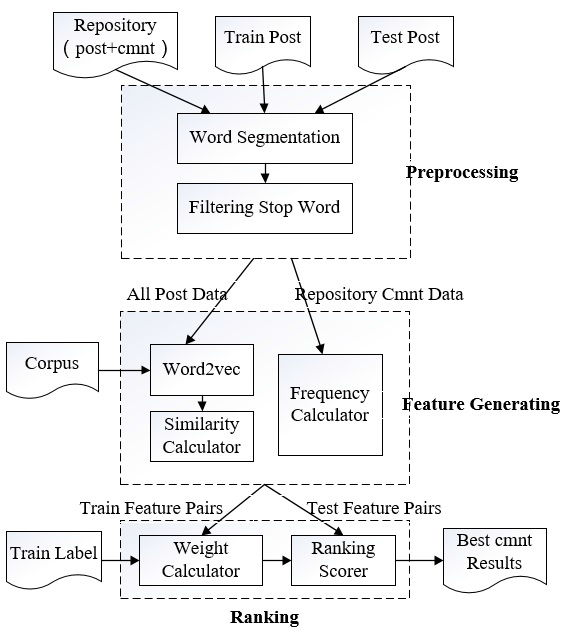
\includegraphics[width=10cm]{Chen_Architecture}
\caption{短对话系统架构} \label{fig:Chen_Architecture}
\end{figure}

如图\ref{fig:Chen_Architecture}所示陈仲夏师兄的系统架构,整个系统分为三个部分,一是将帖子、评论做分词,去停顿词预处理;二是通过的文字上的相似为新帖子在语料库中找出相似的帖子集;三是收集相似帖子集对应的评论集,综合考虑帖子的相似度、评论的频率为候选评论排序选出10个评论并排序。

我们今年的短对话系统继承于陈仲夏师兄的设计,主要区别是在第二部分为新帖子找的相似的帖子上,这也是本文研究的主要目标。除了陈仲夏师兄利用文字上的相似性来关联相似的帖子,我们还想利用图片搜索引擎将短文本视觉化,利用视觉上的相似性来寻找和重新排序相似的帖子。考虑的今年的短文本对话比赛过滤掉了大部分高频的部分,李顶龙同学会对第三部分评论排序部分做相关研究和修改。


%短文本对话是指根据一段短文字,计算机模仿人类给出连贯的有意义的回复。过去文本都是从语料库中找寻合适的回答,   近些年随着机器学习的发展,循环神经网络RNN和长短周期神经网络LSTM的出现文字转向量Word2Vec技术的成熟,文本生成技术是的生成文本回复短对话有种有短文本对话是当下热门的研究方向,以微软小冰、苹果Safari为代表,各家互联网公司都在积极研发对话机器人。现在得到对话问答




